\documentclass[border={0pt 0pt -40pt -40pt}]{standalone}
\usepackage{pgfplots}
\usepackage{tikz}
\usepackage{xcolor}

\begin{document}

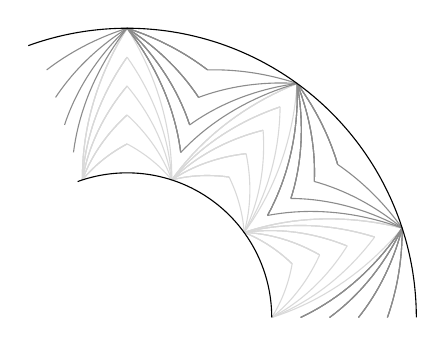
\begin{tikzpicture}
    \begin{axis}[axis lines=none, axis equal,
    xmin=-0.7,xmax=3,
    ymin=-0.1,ymax=3,
    samples=20
    ]

    \foreach \m in {10}{
      \foreach \t in {0.2,0.4,0.6,0.8,1}{
        \foreach \n in {0,...,2}{
          \addplot[gray!30,domain=0:(1/(2* \m ))](
          {cos((\n + \m *x)*360/ \m )*(1+\t *2*( \m  * x ))},
          {sin((\n + \m *x)*360/ \m )*(1+\t *2*( \m  * x ))});
          \foreach \n in {1,...,3}
          \addplot[gray!30,domain=0:(1/(2* \m ))](
          {cos((\n - \m *x)*360/ \m )*(1+\t *2*( \m  * x ))},
          {sin((\n - \m *x)*360/ \m )*(1+\t *2*( \m  * x ))});
        }
      }
      \foreach \t in {0.2,0.4,0.6,0.8}{
        \foreach \n in {0,...,2}{
          \addplot[gray!90,domain=0:(1/(2* \m ))](
          {cos((\n + \m *x)*360/ \m  + 180/ \m )*(2-\t *2*( \m  * x ))},
          {sin((\n + \m *x)*360/ \m  + 180/ \m )*(2-\t *2*( \m  * x ))});
          \foreach \n in {0,...,2}
          \addplot[gray!90,domain=0:(1/(2* \m ))](
          {cos((\n - \m *x)*360/ \m  + 180/ \m )*(2-\t *2*( \m  * x ))},
          {sin((\n - \m *x)*360/ \m  + 180/ \m )*(2-\t *2*( \m  * x ))});
        }
      }
    }

    \addplot[samples=100,domain=0:110]({cos(x)},{sin(x)});
    \addplot[samples=100,domain=0:110]({2*cos(x)},{2*sin(x)});
  \end{axis}
\end{tikzpicture}
\end{document}


